\documentclass{beamer}
\usetheme{CambridgeUS}

\usepackage{tikz}
\usetikzlibrary{shapes, arrows.meta, positioning}

\title{IITH Survey System}
\author{Abhinav Yadav\\
        Beeram Sandya\\
        Prasham Walvekar}

\begin{document}
\maketitle

\begin{frame}{Table of contents}
    \tableofcontents
\end{frame}

\begin{frame}
    \frametitle{Introduction}
    \section{Introduction}
    \begin{enumerate}
        \item Would be form based app
        \item \textbf{Roles:}
              \begin{itemize}
                  \item Surveyor
                  \item Surveyee
              \end{itemize}
        \item Surveyor creates the survey form and sends link to the surveyee
        \item Surveyee fills the form and submits it
        \item Surveyor gets all the responses
        \item Form creator could also get a summary of all the responses (for eg. pie chart for multiple choice responses, line chart for numerical responses, etc.)
        \item App Would support various kinds of responses (more on that later)
        \item No concept of admin. Anyone with IITH account can conduct survey
    \end{enumerate}
\end{frame}


\begin{frame}{User-App interaction}
    \section{User-App interaction}
    \begin{figure}
        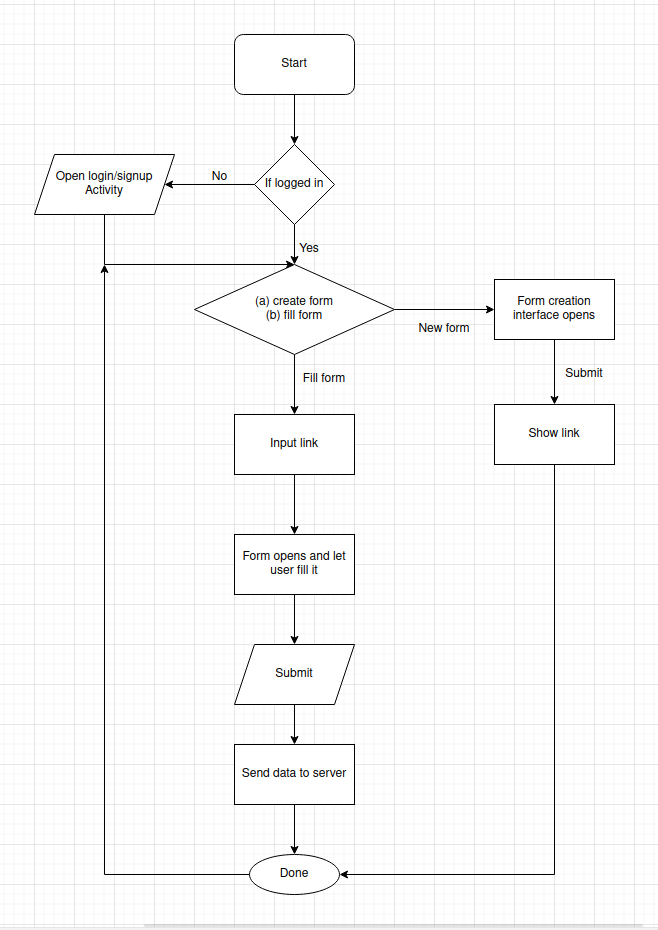
\includegraphics[width=0.45\columnwidth]{images/AppWorking.png}
    \end{figure}
\end{frame}

\begin{frame}[allowframebreaks]{App Internals}
    \section{App Internals}
    \begin{enumerate}
        \item \large Login Activity
              \begin{figure}[h]
                  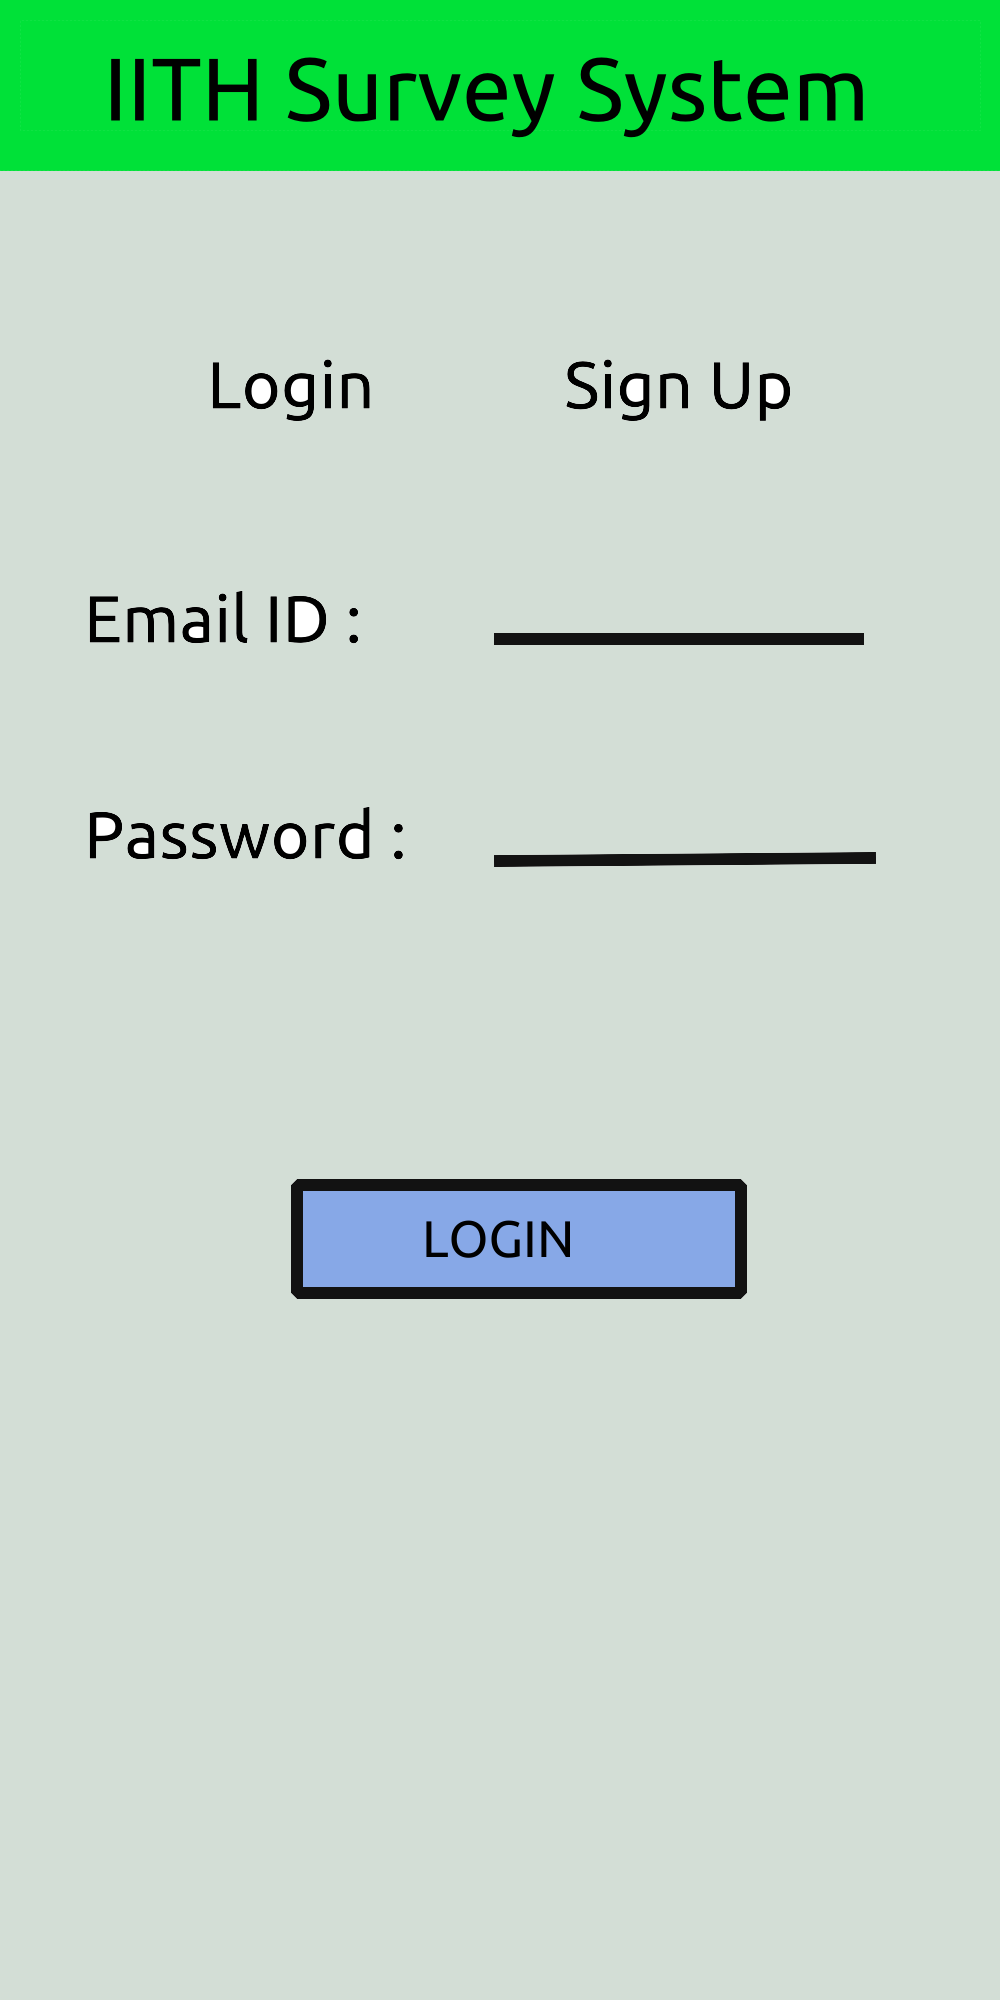
\includegraphics[width=0.2\columnwidth]{images/login.png}
                  \caption{Login}
              \end{figure}
              \pagebreak
        \item \large Home Activity
              \begin{figure}
                  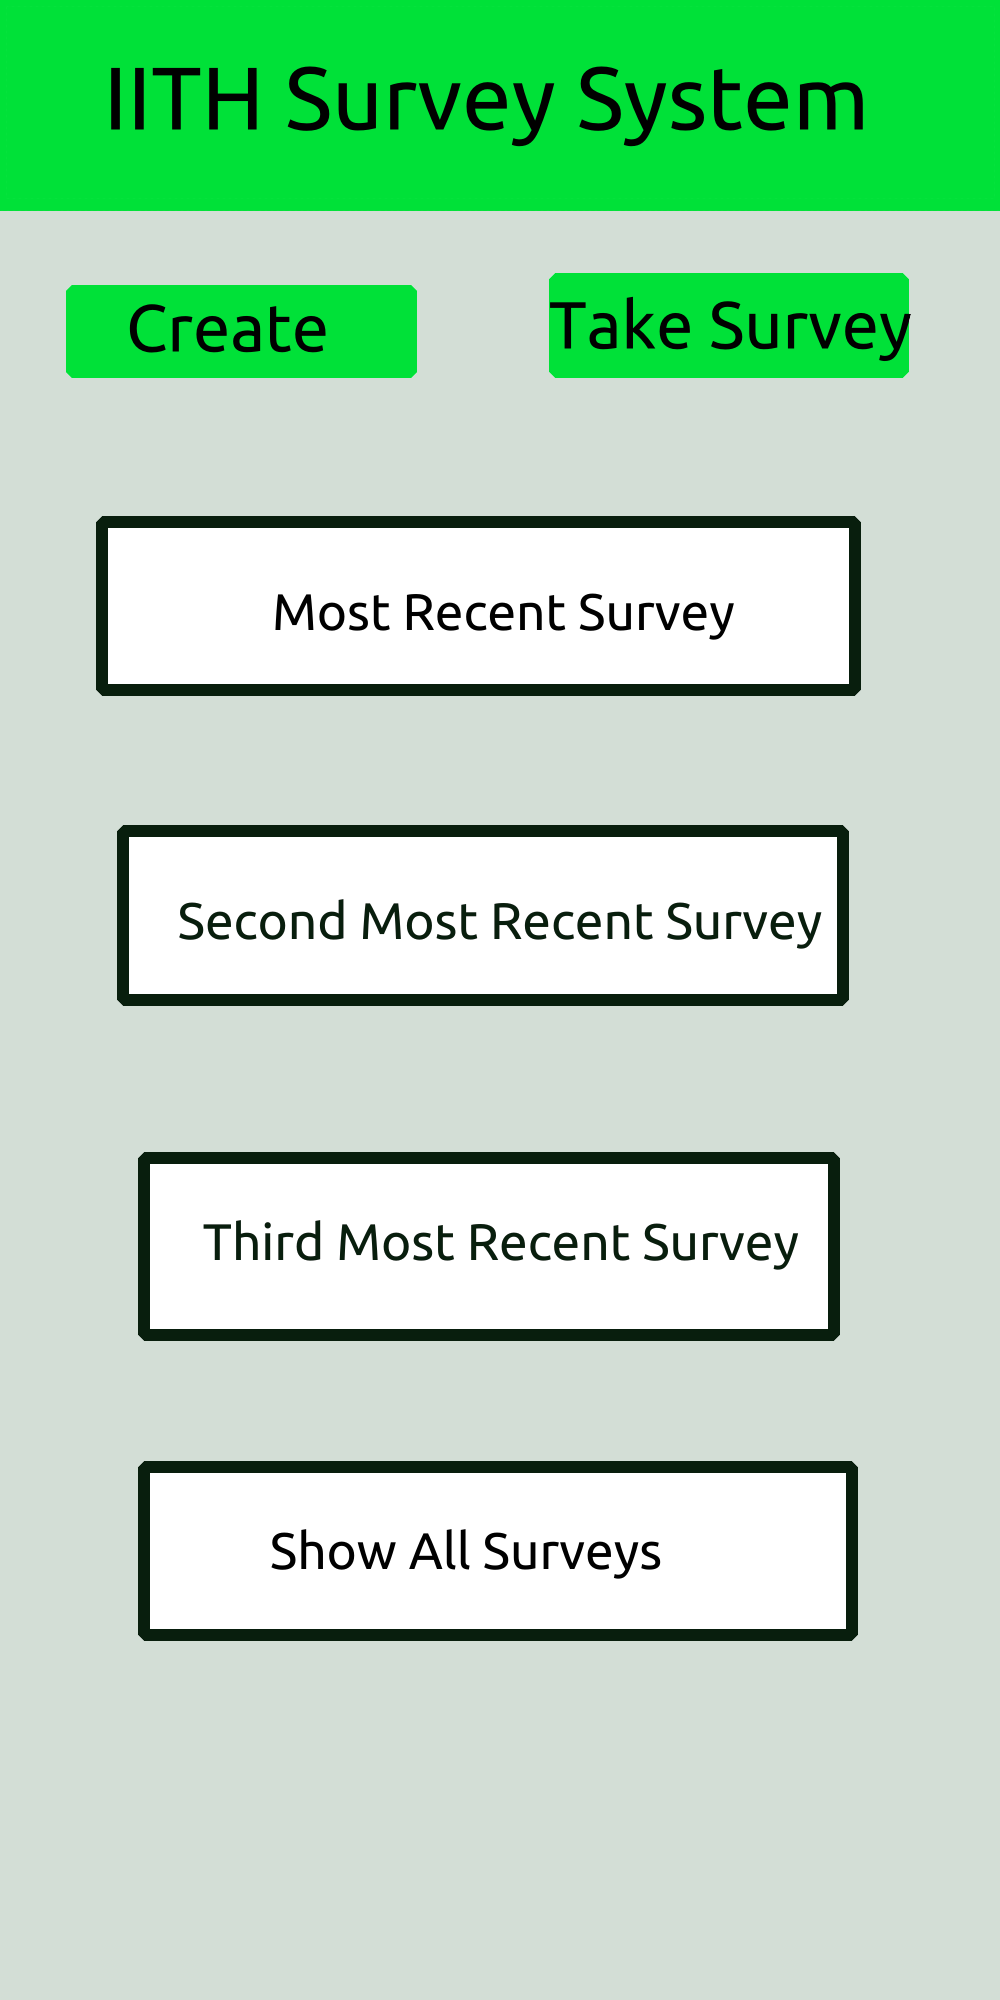
\includegraphics[width=0.2\columnwidth]{images/home.png}
                  \caption{Home}
              \end{figure}

              \pagebreak
        \item \large Form Creation Activity
              \begin{figure}
                  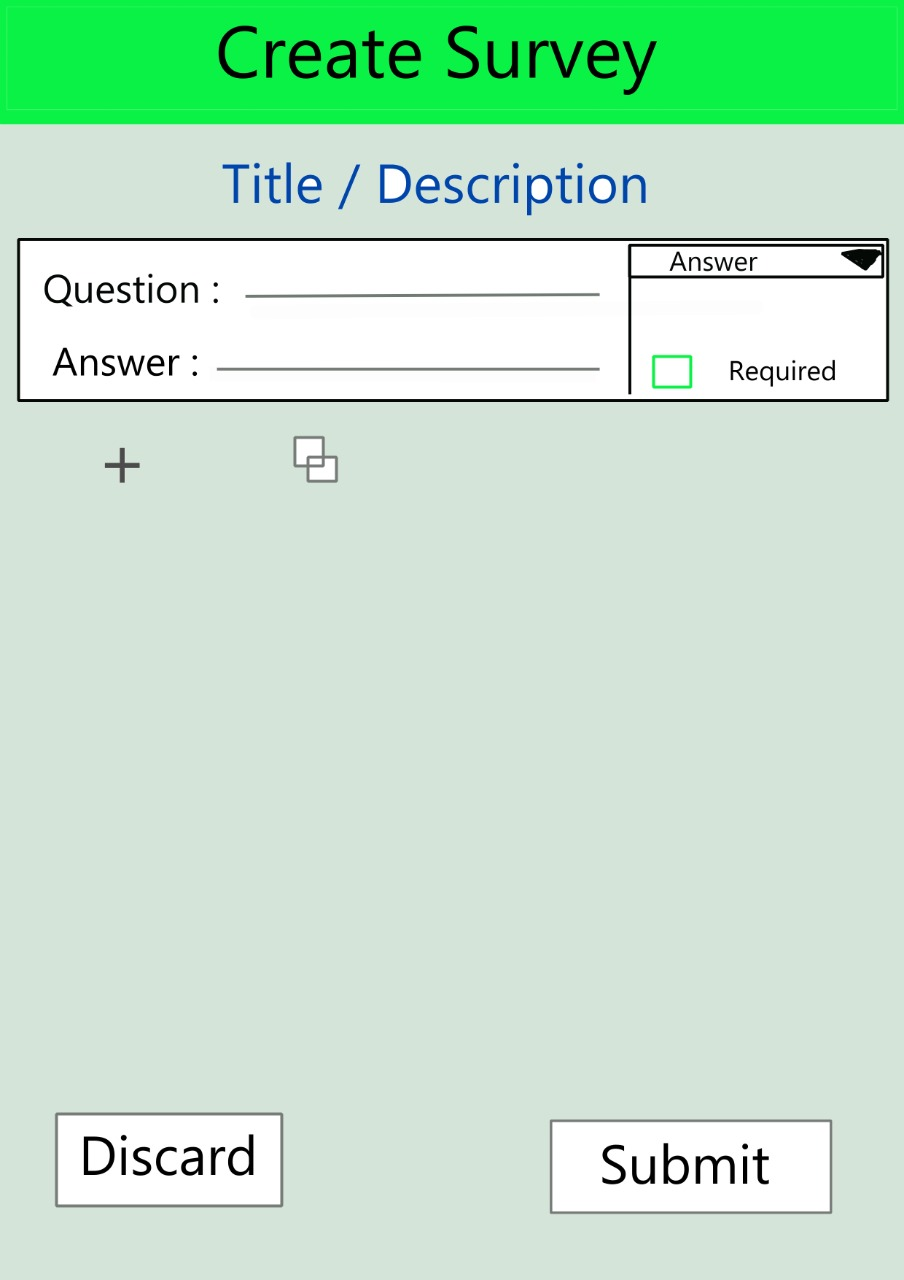
\includegraphics[width=0.25\columnwidth]{images/FormCreation.jpeg}
                  \caption{Form Creation}
              \end{figure}

    \end{enumerate}
\end{frame}

\begin{frame}{Insider view of form creation}
    \section{Insider view of form creation}
    Would consist of questions and answers\\
    \begin{itemize}
        \item Question would contain any one or both
              \begin{itemize}
                  \item Text
                  \item Image
              \end{itemize}

        \item Answer can be any one of following types
              \begin{itemize}
                  \item Text Answer
                  \item Multiple choice with radio buttons
                  \item Multiple choice with check boxes
                  \item Link
                  \item File
                  \item Date
                  \item Time
                  \item Rating
                  \item Rating martrix
              \end{itemize}
    \end{itemize}
\end{frame}

\begin{frame}{Languages and Frameworks to be used}
    \section{Languages and Frameworks to be used}

    \begin{itemize}
        \item Web App
              \begin{enumerate}
                  \item \textbf{Javascript:}
                        \begin{itemize}
                            \item \textbf{reactjs} Logic for working of the Web App
                            \item \textbf{nodejs} The server
                        \end{itemize}
                  \item \textbf{HTML \& CSS:} UI design of the app
                  \item \textbf{MySQL:} Database
              \end{enumerate}
              % \item Android App
              %       \begin{enumerate}
              %           \item \textbf{Java:} Internal working and dynamic UI of the app
              %           \item \textbf{XML:} Static UI design of the app
              %           \item \textbf{nodejs:} For the server
              %           \item \textbf{MySQL:} Database
              %       \end{enumerate}
    \end{itemize}
\end{frame}
\end{document}